% \noindent \begin{table*}[htbp]
%   \centering
%   \begin{tabular}[c]{|l||l|l|l|}
%   %\begin{tabular}[c]{|l||l|l|l|}
%     \hline
%     Embeddings&Classifier (default sklearn settings)&Accuracy\\
%     \hline
%     &&\\
%     GloVe with $\eta$ = 0.001, $\alpha$ = 0.75, nmax = 100, epochs = 10& & \\
%     \hspace{4mm} \textbullet \space 20 features&Logistic regression&0.5965 $\pm$ 0.00197\\
%     \hspace{4mm} &SVM&0.6083 $\pm$ 0.00140\\
%     \hspace{4mm} \textbullet \space 100 features&Logistic regression&0.6159 $\pm$ 0.00069\\
%     \hspace{4mm} &SVM&0.6041 $\pm$ 0.00165\\
%     TF-IDF& & \\
%     \hspace{4mm} \textbullet \space default&Logistic regression&0.8097 $\pm$ 0.00243\\
%     %\hspace{4mm} &Naive Bayes (Multinomial NB)&0.7651 $\pm$ 0.00042\\
%     \hspace{4mm} &SVM&0.7914 $\pm$ 0.00039\\
%     \hline
%   \end{tabular}
%   \vspace{3mm}
%   \caption{Numerical word representation models on small data set}
%   \label{Baselines_table}
% \end{table*}

\begin{table*}[htpb]
\centering
\resizebox{1.5\columnwidth}{!}{
\tiny\tiny
\begin{tabular}[c]{{l}c*{1}c} 
\hline
\rule{0pt}{2mm}
\textbf{Embeddings}&\textbf{Classifier}&\textbf{Accuracy}\\
\hline
\rule{0pt}{3mm}
GloVe with $\eta$ = 0.001, $\alpha$ = 0.75, nmax = 100, epochs = 10& & \\
\rule{0pt}{2mm}
\hspace{4mm} \textbullet \space 20 features&LogReg&0.5965 $\pm$ 0.00197\\
    \hspace{4mm} &SVM&0.6083 $\pm$ 0.00140\\
\rule{0pt}{2mm}
    \hspace{4mm} \textbullet \space 100 features&LogReg&0.6159 $\pm$ 0.00069\\
    \hspace{4mm} &SVM&0.6041 $\pm$ 0.00165\\
TF-IDF& & \\
\rule{0pt}{1mm}
    \hspace{4mm} \textbullet \space default&LogReg&0.8097 $\pm$ 0.00243\\
    \hspace{4mm} &SVM&0.7914 $\pm$ 0.00039\\
    \hline
\end{tabular}
}
\caption{Numerical word representation models on small data set. Classifiers are from scikit-learn, with default settings.}
\label{Baselines_table}
\end{table*}

In this section we specify the results obtained for each of the methodologies discussed, and the analysis performed in order to construct our final sentiment analysis model.
%\textbf{TODO: THE FOLLOWING ARE NOOOOOT RESULTS!!! PUT THEM BACK TO METHODOLOGY. THOSE ARE NOT METHODOLOGY EITHER...OUR METHODOLOGY IS A GENERALIZED TEXT}
\subsection{Feature generation}
To select the best model for generating numerical word representations, we compare the GloVe word embedding, with both 20 and 100 features per word, with the default instance of TF-IDF from \textit{scikit-learn}\cite{scikit-learn}.
To obtain a first insight into the performances of the models, we perform the training of the obtained word-to-vector matrix and word-frequency-based feature matrix using the LogReg and SVM classifiers from \textit{scikit-learn} without any hyperparameter optimization. 
As it is shown in Table~\ref{Baselines_table}, the best classification results of the raw data are obtained using TF-IDF word vectors. 
We therefore proceed using TF-IDF to optimize data pre-processing and hyperparameter optimization steps for LogReg and SVM classifiers in order to improve their accuracy.
Moreover, the accuracy of a classifier increases with the dataset size, as shown in Fig. \ref{fig:dataset}.\\
% \vspace{0.3cm}
\begin{figure}[h]
%    	\begin{subfigure}[]{0.50\textwidth}
        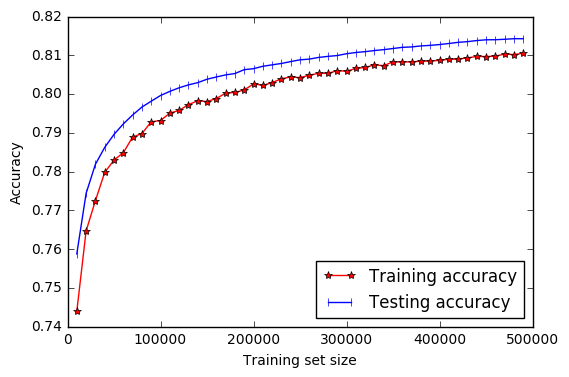
\includegraphics[width=0.965\columnwidth]{plots/data_set_size_vs_accuracy.png}
            \caption{Effect of dataset size on accuracy as observed on test set with default TF-IDF LogReg model.}\label{fig:dataset}
%             \caption{\small}
%             \label{fig:a}
%     \end{subfigure}
    ~ %add desired spacing between images, e. g. ~, \quad, \qquad, \hfill etc. 
      %(or a blank line to force the subfigure onto a new line)
%       \vspace*{-1.5mm}
%     \begin{subfigure}[]{0.50\textwidth}
%         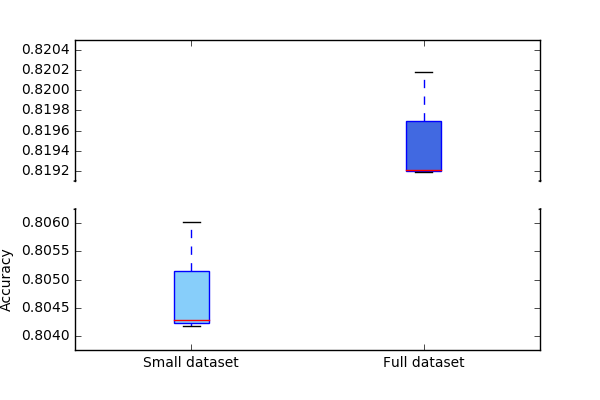
\includegraphics[width=\columnwidth]{plots/nicely_cut_colored.png}
%             \caption{\small}
%             \label{fig:b}
%     \end{subfigure}
    ~ %add desired spacing between images, e. g. ~, \quad, \qquad, \hfill etc. 
    %(or a blank line to force the subfigure onto a new line)
    \
\end{figure}
\vspace{-1cm}
\subsection{Pre-processing}
We now show the additional pre-processing steps, in an aggregating manner, used to obtain the best classification accuracy for each of the aforementioned classifiers.
The baseline pre-processor is referred to the received dataset (having applied the pre-processing steps described in section \ref{preproIII}).
\subsubsection{Dummy}
The baseline classifier is a random classifier that is evaluated on the received dataset without any pre-processing.
As expected, the accuracy of such classifier is around $50\%$. Specifically, $0.5018 \pm 0.0019$ for a 3-fold CV.
\subsubsection{LogReg}
For each additional pre-processing step, a LogReg classifier (with default regularization parameter \texttt{$C$=1}) is trained. 
The pre-processing steps that yielded improvements on test accuracy are listed in Table \ref{tab:logreg_table}. 
Other pre-processing steps yielded lower test set accuracies.
\vspace{-0.19cm}
\begin{table}[H]
\centering
\resizebox{\columnwidth}{!}{
% \tiny
\begin{tabular}{{l}c*{2}c} 
\hline
	            & \textbf{train} & \textbf{test} & \textbf{change} \\
\hline
\rule{0pt}{3mm}
base			& 0.8048$\pm$0.0009	& 0.8097$\pm$0.0024 	& 0.00$\%$	\\
+repeating letters & 0.8227$\pm$0.0015 & 0.8271$\pm$0.0015
    & 1.74$\%$  \\
+stem           & 0.8254$\pm$0.0020	& 0.8303$\pm$0.0025 	& 0.30$\%$ 	\\
+remove \# & 0.8258$\pm$0.0022	& 0.8306$\pm$0.0024 	& 0.03$\%$ 	\\
+2-grams        & 0.8372$\pm$0.0013	& 0.8457$\pm$0.0046 	& 1.51$\%$ 	\\
\hline
\end{tabular}
}
\caption{\label{tab:logreg_table}Best pre-processing steps for default LogReg.}
\end{table}
% \vspace{-1.3cm}
% \vspace{0.3cm}
The improvement observed by replacing repeating letters is reflective of the way people express their emotions in a textual form.
\vspace{-0.1cm}
\subsubsection{SVM}
The preprocessing steps that yielded improvements on test accuracy for SVM are listed in Table \ref{tab:svm_table}.
\vspace{-0.19cm}
\begin{table}[H]
\centering
\resizebox{\columnwidth}{!}{
% \tiny
\begin{tabular}{{l}c*{2}c} 
\hline
	            & \textbf{train} & \textbf{test} & \textbf{change} \\
\hline
\rule{0pt}{3mm}
base			&0.7908$\pm$0.0016  	&0.7918$\pm$0.0005 	&0.00$\%$			\\
+repeating letters          &0.8142$\pm$0.0011 	&0.8163$\pm$0.0010 	&2.45$\%$	 	\\
+stem        &0.8142$\pm$0.0020 	&0.8171$\pm$0.0014	&0.08$\%$	 	\\
%+remove \#   &0.8149 	&0.8168 	& 1 	\\
+2-grams   &0.8178$\pm$0.0018 	&0.8198$\pm$0.0010 	&0.27$\%$	 	\\
\hline
\end{tabular}
}
\caption{\label{tab:svm_table}Best pre-processing steps for default SVM.}
\end{table}
\vspace{-0.5cm}
\subsubsection{MNB}
The preprocessing steps that yielded improvements on test accuracy are listed in Table \ref{tab:MNB_table}.
% \vspace{0.3cm}
\begin{table}[H]
\centering
\resizebox{\columnwidth}{!}{
% \tiny
\begin{tabular}{{l}c*{2}c} 
\hline
	            & \textbf{train} & \textbf{test} & \textbf{change} \\
\hline
\rule{0pt}{3mm}
base			&0.7642$\pm$0.0011  	&0.7650$\pm$0.0004 	& 0.00$\%$		\\
%+repeating letters  &0.7642  	&0.7650 	& 0 	\\
%+stem      &0.7642  	&0.7650 	& 1 	\\
%+remove \#  &0.7642  	&0.7650  	& 1 	\\
%+emoticon \#  &0.7638  	&0.7628  	& 1 	\\
+replacing not	&0.7664$\pm$0.0015  	&0.7671$\pm$0.0003  	& 0.21$\%$ 	\\
+english stop words	&0.7668$\pm$0.0009  	&0.7675$\pm$0.0003  	& 0.04$\%$	\\
+2-grams   &0.7846$\pm$0.0013	&0.7903$\pm$0.0028	& 2.35$\%$  	\\
\hline
\end{tabular}
}
\caption{\label{tab:MNB_table}Best pre-processing steps for default MNB.}
\end{table}
% \vspace{0.3cm}
A pictorial representation comparing the best pre-processing steps for each classifier is given in Fig. \ref{fig:classifiers}.
% \vspace{0.3cm}
\begin{figure}[H]
	\centering
	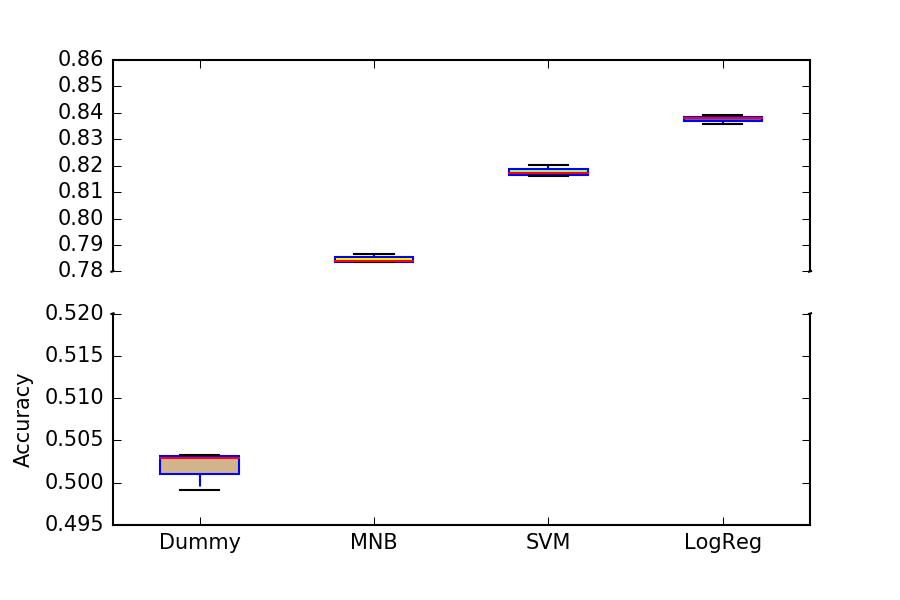
\includegraphics[width=\columnwidth]{plots/Classifiers_boxplots2.png}
    \caption{Accuracies for each investigated classifiers (default hyperparameters from \textit{scikit-learn} modules) including its optimal pre-processing.}
    \label{fig:classifiers}
\end{figure}
% \vspace{0.3cm}
It is thus clear that replacing multiple occurrences of two words improves the classification accuracy of LogReg and SVM. Another determining hyperparamter is the \textit{n-grams} while feature generation. 
%\ref{fig:all_models_boxplots} 
\subsection{Hyperparameter optimization}
The \textit{CountVectorizer()} and \textit{TfidfTransfromer()} from \textit{scikit-learn} have multiple hyperparameters that can be tuned. 
A first hyperparameter is \texttt{N-gram}, already described in the Methodology section. 
Other hyperparameters are \texttt{max\textunderscore df}, a threshold to cut off highly frequent words; and \texttt{min\textunderscore df}, a threshold to clip off very rare words. 
Moreover, the maximal amount of features, \texttt{max\textunderscore features}, can be set. 
Another hyperparameter is the inverse L2 regularization strength (\texttt{C}) of the LogReg. \\
In order to search through the complete landscape of each hyperparameter, we first apply a random search using  \textit{scikit-learn}'s \textit{RandomSearchCV()}, on a wide range of hyperparameters to get an initial idea of the optimal parameters for the full dataset. 
The returned values are reported in Table \ref{tab:coarse_hyper} and give an accuracy of $0.8686 \pm 0.0023$ on the full dataset.
% \begin{table}[H]
% \centering
% \resizebox{.5\columnwidth}{!}{
% % \tiny
% \begin{tabular}{{l}c} 
% \hline
% \rule{0pt}{2mm}
% \textbf{hyperparameter} & \textbf{value}\\
% \hline
% \texttt{max\_features}			&$None$ \\
% \texttt{ngram\_range}			&$(1,3)$ \\
% \texttt{max\_df}				&$\approx 0.9261$ \\
% \texttt{min\_df}				&$4$ \\
% \texttt{C}						&$\approx 2.1544$ \\
% \hline
% \end{tabular}
% }
% \caption{\label{tab:coarse_hyper}Hyperparameters returned by coarse RandomSearchCV().}
% \end{table}

% \vspace{0.3cm}
\begin{table}[!htb]

    \begin{subtable}{.48\linewidth}
      \caption{\label{tab:coarse_hyper}}
      \centering
       \begin{tabular}{{l}c} 
\hline
\rule{0pt}{2mm}
\textbf{hyperparameter} & \textbf{value}\\
\hline
\texttt{max\_features}			&$None$ \\
\texttt{ngram\_range}			&$(1,3)$ \\
\texttt{max\_df}				&$\approx 0.9261$ \\
\texttt{min\_df}				&$4$ \\
\texttt{C}						&$\approx 2.1544$ \\
\hline
\end{tabular}
    \end{subtable}%
    \begin{subtable}{.48\linewidth}
      \centering
       \caption{\label{tab:fine_hyper}}
        \begin{tabular}{{l}c}
\hline
\rule{0pt}{2mm}
\textbf{hyperparameter} & \textbf{value}\\
\hline
\texttt{max\_features}			&$None$ \\
\texttt{ngram\_range}			&$(1,3)$ \\
\texttt{max\_df}				&$\approx 0.9261$ \\
\texttt{min\_df}				&$4$ \\
\texttt{C}						&$3.41$ \\
\hline
\end{tabular}
    \end{subtable} 
        \caption{Hyperparameters returned by (a) coarse RandomSearchCV() and (b) fine sampling around the optimal range.}

\end{table}
% \vspace{0.3cm}
We then perform a fine-grain search on the small dataset to optimize the hyperparameter \texttt{C} for Logistic Regression. 
Fig. \ref{fig:C_Landscape} illustrates the testing accuracy peak of $0.8534 \pm 0.0039$ at around $\texttt{C} = 3.41$ on the small dataset that yield an accuracy of $ 0.8739 \pm 0.0017$ on the full dataset after 3-fold CV.
The final hyperparameters are then the ones specified in Table \ref{tab:fine_hyper} with \texttt{1783165} features.

%\textbf{We still have to write about the ROC curve!}
To analyze the classification performance of our classification system, we plot the \textit{receiver operating characteristic (ROC) curve} \ref{fig:ROC}. 
This is the true positive rate against the false positive rate for the different possible cut-points. 
Generally, the closer the curve to the left upper corner of the ROC space, the more accurate the classification; and the closer the curve to the diagonal, the less accurate the classification. 
Therefore, the \textit{area under the curve (AUC)} is a measure of classification accuracy.
One can see that the AUC of the mean ROC over three folds is $0.92 \pm 0.0047$, showing that our classification holds an accuracy of $92\%$.
%TF-IDF: ngram, maxdf, mindf, max features
%Logistic regression holds multiple hyperparameters one needs to tune. C